\documentclass[12pt]{article}
\usepackage[utf8]{inputenc}
\usepackage{color}
\usepackage{graphicx}

\begin{document}
\title{Novel Video Analytics and Tapestry (NVAT)}
\color{black}
\author{ V Alekhya, Nadimpalli Vineetha, Tarun Rajnish, Mohammed Talha Zubair \\Project Guide: Dr Suryaprasad J}
\maketitle

\noindent
\section{Problem Definition}
Video content analysis (also Video content analytics, VCA) is the capability of automatically analyzing video to detect and determine temporal and spatial events. Detecting intrusions and trespassers through video data from CCTV surveillance cameras forms one of the major domains under video analytics and is important to ensure safety and security.
Here, we attempt to process the data obtained from CCTV footage via various static and dynamic video stitching techniques in order to detect unwanted access. We work out and display a timeline depicting the path traveled, computed from the feed of multiple cameras and do so in an optimized, efficient and simplified manner.
\newline

\textit{Key Terms: Video Analytics, Surveillance, Artificial Intelligence, Image Processing, Editing}

\section{Introduction}

Before the days of computerized video footage analysis, humans had to do the bulk of the work which included assessing hours of video data. Any related information had to be assessed and then passed on to the next level for various purposes. The process was tedious and cumbersome as well as included chances of human error or oversight. Human operators, can be highly ineffective at capturing and processing video data during extended periods, a phenomenon known as “in-attentional blindness". According to recent study, it was discovered that, on an average it is impossible for someone to concentrate for more than twenty minutes on the screen. In addition,there are high labor costs associated with staffing to monitor CCTV feeds and retrieve, manage and store video content. Thus arose a need to eliminate human intervention for the processing of surveillance data and the natural transition was to make the whole process computerized in order to make it faster and more efficient and thus, computerized video analytics was born.
\newline

\noindent
Video content analysis is the capability of automatically analyzing video to detect and determine temporal and spatial events. This technical capability is used in a wide range of domains including entertainment, health-care, retail, automotive, transport, home automation, flame and smoke detection, safety and security. We would be focusing on its application especially in surveillance camera networks.
\newline

\noindent
The primary function of a VMD (Video Motion Detection Device) is to relieve CCTV operators from the stress of monitoring one or many screens of information that may not change for long periods. The VMD system will be monitoring all the cameras in its system, and only reacting when there is suspicious activity in one of the scenes. The idea of VMD systems is that the processor is continuously monitoring all the cameras in the system. During this time, the, operator may select or sequence cameras using the conventional switching system. When activity in any camera occurs that the VMD system interprets as an intruder, the alarmed camera is immediately switched to a blank monitor and a warning sounded to alert the operator. The operator’s attention, is therefore, immediately focused on the camera covering the alarm

\section{Literature Survey}

Andrew A. Adams and James M. Ferryman \cite{num:1} discuss the three stages of a surveillance system. The first stage for people and/or object monitoring is detection and classification which consists of localizing new objects entering the surveillance area. Particular attention recently has been given to person detection with state-of-the-art methods based on Histogram-of Gradients (HOG) feature in combination with other features, and classifier learning (Dollár et al., 2012). Random forests and ferns have now established themselves as a fast and reliable appearance descriptor for object classification (Evans et al., 2012). Classifier grids, in which a separate classifier is trained for each image location, have also been shown to be a powerful method for object detection. An understanding of the type of object identified can then allow the vision system to more accurately track the object through the scene which is part of the next stage. The final stage of a surveillance system is to attempt to understand the behaviors of tracked objects and the interactions between objects, and with the environment. A common approach is to apply a set of predetermined spatio-temporal rules that are correlated to what operators would interpret as “interesting”.
\newline

\noindent
White Paper Agent Video Intelligence \cite{num:2} introduces an architectural approach to Video Analytics, "Agent Vi’s Distributed Implementation Agent Vi", called “Image Processing over IP networks” (IPoIP™). With Agent Vi’s architecture, the Video Analytics task is distributed between the edge device (which may be an IP camera or encoder) and a server. This approach optimizes the workload on the edge device and server and yields high quality analytics performance. A key benefit to Agent Vi’s distributed architecture is that a single server can run comprehensive Video Analytics functions on hundreds of cameras simultaneously. This hardware efficient camera-to server ratio is achieved without compromising on the range and performance of the analytics functionality, which makes it especially beneficial for large scale surveillance installations.
\newline

\noindent
Frost \& Sullivan mention in their white paper \cite{num:3} that the core of IBM's Intelligent Video Analytics solution deals with the application of analytic and information management tools to the available video data.
It can process the video data in real time to extract events (activities in the camera’s field of view) and classify the events or objects in them in multiple ways, including generating metadata on them.
Analytics can then be applied for the classification of data and metadata and assessing if the event falls within a predefined condition of interest i.e an intruder in this case.
The solution’s metadata capability enables a large number and variety of analytics to be applied to activities. Thus, metadata tagging, one of the most key capabilities of IBM's Intelligent Video Analytics solution, is one of the techniques we plan to use.

\section{Objective}

Our objective can be divided into 3 steps.

We initially integrate continuous live CCTV footage (Cameras C1, C2, ...) with an existing Video Editing Software. Our Artificial Intelligence (AI) algorithm running on the server, monitors this feed and spots any dynamic movements (intruders) on the static backdrop of the camera. (See Fig 1)

The movements are captured in a sequence of snap shots and the software attempts to stitch the array of snap shots together using database assistance to retrieve and store video clips to generate a trespassing path. This path is in turn re-generated as a graphic mapping of the intruder on a blueprint of the compound/campus.

We also add a User Interface (accessed via a computer or a phone) where the user can select from a bunch of editing, selection and processing options available in the menu to work on the images or video.
\newline

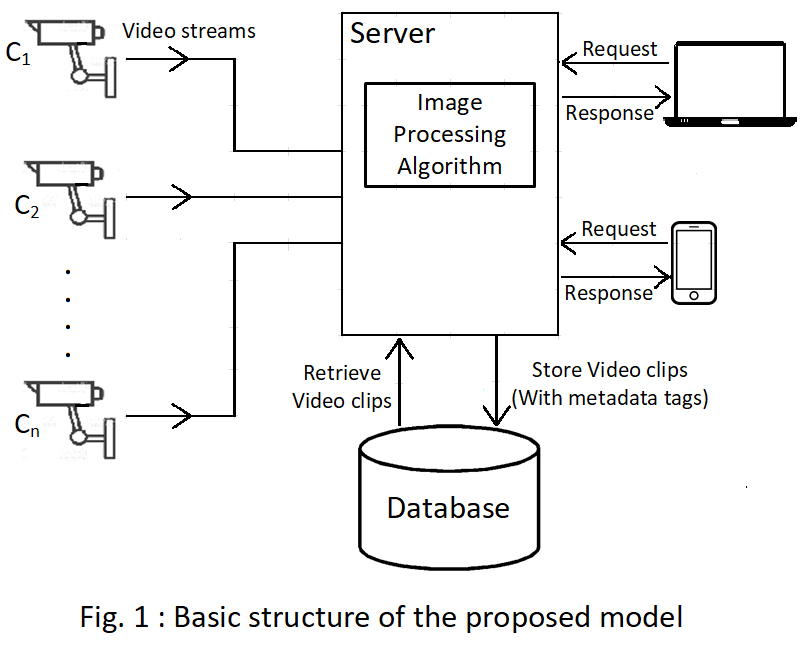
\includegraphics[width=\textwidth]{HighLevelBlockDiagram.png}


\section{Methodology}
To be done

%\section{Model}
%To be done

\section{Assumptions}
To be done

\section{Outcomes}
To be done

\bibliography{Bibliography}
\bibliographystyle{ieeetr}

\end{document}
